
\exercise[(skewed leapfrog)]{10.3}

Suppose $a>0$ and consider the following {\it skewed leapfrog} method for
solving the advection equation $u_t + au_x = 0$:
\eqlex{a}
U_j^{n+1} = U_{j-2}^{n-1}  - \left(\frac{ak}{h} - 1\right) (U_j^n -
U_{j-2}^n).
\end{equation}
The stencil of this method is
\vskip 5pt
\hfil\epsfig{file=figs/skewedlfstencil.eps,width=1.5in}\hfil
\vskip 5pt

Note that if $ak/h \approx 1$ then this stencil roughly follows the
characteristic of the advection equation and might be expected to be more
accurate than standard leapfrog.  (If $ak/h = 1$ the method is exact.)


\begin{enumerate}

\item What is the order of accuracy of this method?

\item For what range of Courant number $ak/h$ does this method satisfy the
CFL condition?

\item Show that the method is in fact stable for this range of Courant
numbers by doing von Neumann analysis.  
{\bf Hint:} Let $\gamma(\xi) = e^{i\xi h}g(\xi)$ and show that $\gamma$
satisfies a quadratic equation closely related to the equation (10.34)
that arises from a von Neumann analysis of the leapfrog method.

\end{enumerate}


